% This file was created with tikzplotlib v0.10.1.
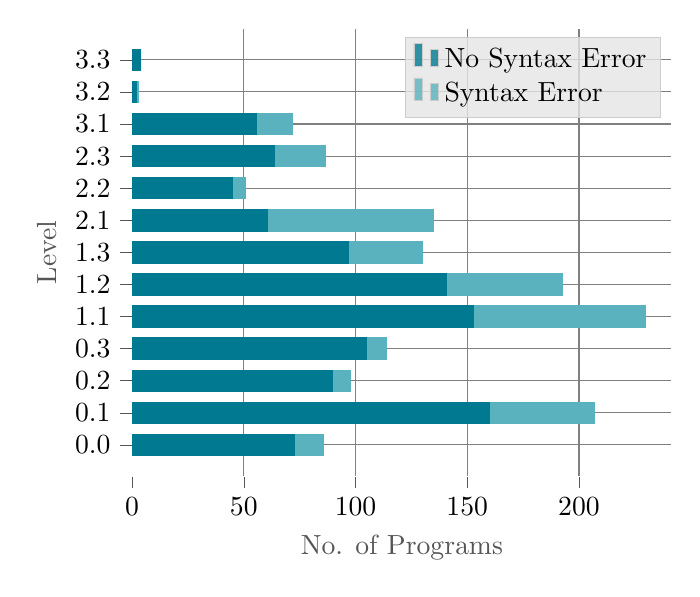
\begin{tikzpicture}

\definecolor{dimgray85}{RGB}{85,85,85}
\definecolor{gainsboro229}{RGB}{229,229,229}
\definecolor{gray}{RGB}{128,128,128}
\definecolor{lightgray204}{RGB}{204,204,204}
\definecolor{mediumaquamarine89178189}{RGB}{89,178,189}
\definecolor{teal0121145}{RGB}{0,121,145}

\begin{axis}[
axis line style={white},
legend cell align={left},
legend style={fill opacity=0.8, draw opacity=1, text opacity=1, draw=lightgray204, fill=gainsboro229},
tick align=outside,
tick pos=left,
x grid style={gray},
xlabel=\textcolor{dimgray85}{No. of Programs},
xmajorgrids,
xmin=0, xmax=241.5,
xtick style={color=dimgray85},
y grid style={gray},
ylabel=\textcolor{dimgray85}{Level},
ymajorgrids,
ymin=-0.985, ymax=12.985,
ytick style={color=dimgray85},
ytick={0,1,2,3,4,5,6,7,8,9,10,11,12},
yticklabels={0.0,0.1,0.2,0.3,1.1,1.2,1.3,2.1,2.2,2.3,3.1,3.2,3.3}
]
\draw[draw=none,fill=teal0121145,very thin] (axis cs:0,-0.35) rectangle (axis cs:73,0.35);
\addlegendimage{ybar,ybar legend,draw=none,fill=teal0121145,very thin}
\addlegendentry{No Syntax Error}

\draw[draw=none,fill=teal0121145,very thin] (axis cs:0,0.65) rectangle (axis cs:160,1.35);
\draw[draw=none,fill=teal0121145,very thin] (axis cs:0,1.65) rectangle (axis cs:90,2.35);
\draw[draw=none,fill=teal0121145,very thin] (axis cs:0,2.65) rectangle (axis cs:105,3.35);
\draw[draw=none,fill=teal0121145,very thin] (axis cs:0,3.65) rectangle (axis cs:153,4.35);
\draw[draw=none,fill=teal0121145,very thin] (axis cs:0,4.65) rectangle (axis cs:141,5.35);
\draw[draw=none,fill=teal0121145,very thin] (axis cs:0,5.65) rectangle (axis cs:97,6.35);
\draw[draw=none,fill=teal0121145,very thin] (axis cs:0,6.65) rectangle (axis cs:61,7.35);
\draw[draw=none,fill=teal0121145,very thin] (axis cs:0,7.65) rectangle (axis cs:45,8.35);
\draw[draw=none,fill=teal0121145,very thin] (axis cs:0,8.65) rectangle (axis cs:64,9.35);
\draw[draw=none,fill=teal0121145,very thin] (axis cs:0,9.65) rectangle (axis cs:56,10.35);
\draw[draw=none,fill=teal0121145,very thin] (axis cs:0,10.65) rectangle (axis cs:2,11.35);
\draw[draw=none,fill=teal0121145,very thin] (axis cs:0,11.65) rectangle (axis cs:4,12.35);
\draw[draw=none,fill=mediumaquamarine89178189,very thin] (axis cs:73,-0.35) rectangle (axis cs:86,0.35);
\addlegendimage{ybar,ybar legend,draw=none,fill=mediumaquamarine89178189,very thin}
\addlegendentry{Syntax Error}

\draw[draw=none,fill=mediumaquamarine89178189,very thin] (axis cs:160,0.65) rectangle (axis cs:207,1.35);
\draw[draw=none,fill=mediumaquamarine89178189,very thin] (axis cs:90,1.65) rectangle (axis cs:98,2.35);
\draw[draw=none,fill=mediumaquamarine89178189,very thin] (axis cs:105,2.65) rectangle (axis cs:114,3.35);
\draw[draw=none,fill=mediumaquamarine89178189,very thin] (axis cs:153,3.65) rectangle (axis cs:230,4.35);
\draw[draw=none,fill=mediumaquamarine89178189,very thin] (axis cs:141,4.65) rectangle (axis cs:193,5.35);
\draw[draw=none,fill=mediumaquamarine89178189,very thin] (axis cs:97,5.65) rectangle (axis cs:130,6.35);
\draw[draw=none,fill=mediumaquamarine89178189,very thin] (axis cs:61,6.65) rectangle (axis cs:135,7.35);
\draw[draw=none,fill=mediumaquamarine89178189,very thin] (axis cs:45,7.65) rectangle (axis cs:51,8.35);
\draw[draw=none,fill=mediumaquamarine89178189,very thin] (axis cs:64,8.65) rectangle (axis cs:87,9.35);
\draw[draw=none,fill=mediumaquamarine89178189,very thin] (axis cs:56,9.65) rectangle (axis cs:72,10.35);
\draw[draw=none,fill=mediumaquamarine89178189,very thin] (axis cs:2,10.65) rectangle (axis cs:3,11.35);
\draw[draw=none,fill=mediumaquamarine89178189,very thin] (axis cs:4,11.65) rectangle (axis cs:4,12.35);
\end{axis}

\end{tikzpicture}
